Resolution studies are used to characterize the precision of a timing reconstruction method. The time resolution is determined by the difference in the times of two recorded hits ( rehit ) in a crystal from a pair of crystals in which the rechits should have been produced simultaneously. As shown in Figure \ref{trm_local_global_xstal}, two methods of selecting this pair of crystals are used. The first method selects for a pair of adjacent crystals that have similar energies to measure a "local resolution".  The "local resolution" is used to characterize the single crystal time resolution with, or without, the effects of delays due to the read out unit electronics. The second method selects for a pair of rechits that correspond to hits generated by electrons from a $Z\rightarrow e^{+}e^{-}$ process.  This second method selects for a "global resolution" which is used to characterize time resolutions typically obtained in physics analyses.
%These two sub cases are referred to as "same read out unit" ( SRU ) in the case where both crystal share the same read out electronics, and "different read out unit" ( DRU ) where the two crystal straddle the boarder between two different read out units.  

\begin{figure}[htbp]
\begin{center}
\resizebox{0.7\textwidth}{!}{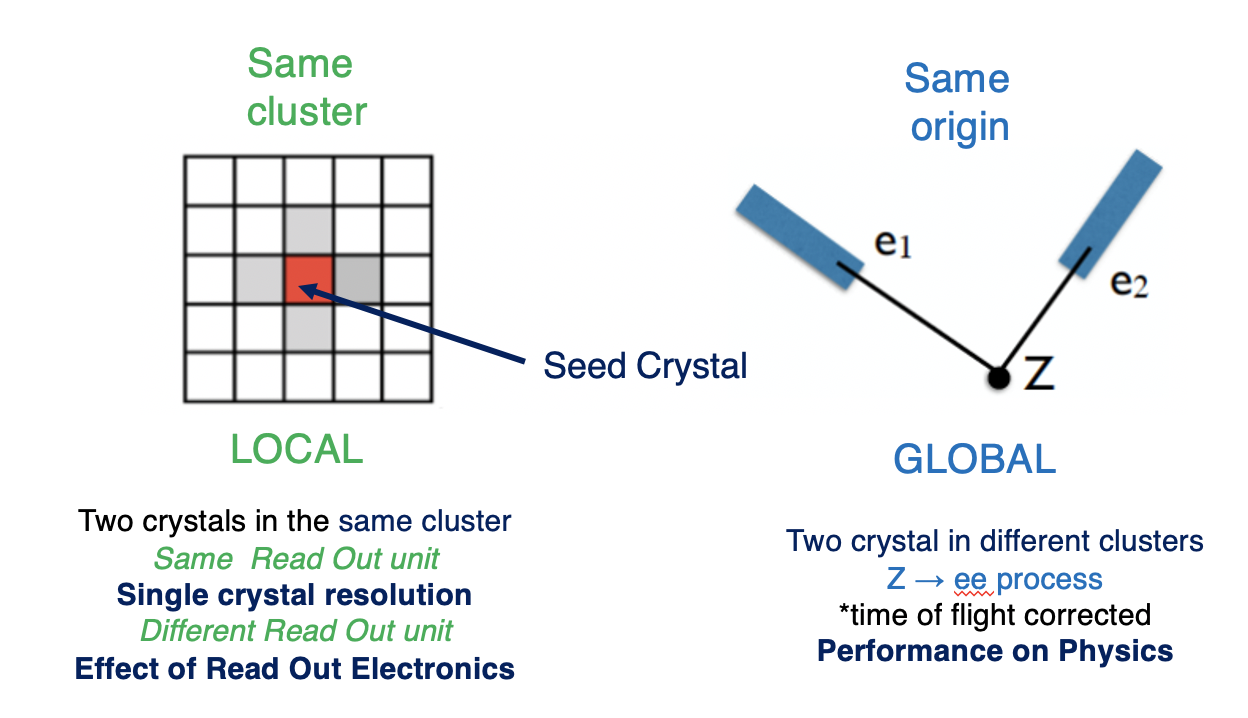
\includegraphics{fig/sec_method/Local_global_crystals.png}}
\caption{The two methods of selecting pairs of crystals to use in determining the time resolution. In a local resolution, used to characterize the single crystal time resolution and the effects of delays due to the read out unit electronics, two adjacent crystals in the same cluster are selected. For a global resolution, used to characterize time resolutions typically obtained in physics analyses, two crystals in different clusters that corresponded to the electrons from a $Z\rightarrow e^{+}e^{-}$ process are selected.} 
\label{trm_local_global_xstal}
\end{center}
\end{figure} 

For a local resolution, shown on the right in Figure \ref{trm_local_global_xstal}, rechits for a pair of crystals from the cluster of crystal that form an EG candidate are selected. The pair of crystal are required to be the seed crystal of the EG candidate and an adjacent crystal in either the $\eta$ or $\phi$ directions for which the rechit energy of the second crystal is required to be within 20\% of the energy of the rechit in the seed crystal. The selected EG candidates from which the crystal pair is taken is required to have the semi-minor axis of the second moment of the crystal cluster geometrical distribution (smin) to be $<$ 0.3, and the semi-minor axis (smaj) to be $<$ 0.5. When more than one EG candidate has a qualifying crystal pair in a collision event, the EG candidate with the largest momentum in the event is selected.  Local resolutions are further divided into a case where both crystals share the same readout electronics, referred to as a 'Same RO Unit' resolution, and a case where the crystals in the pair have a different readout unit, referred to as 'Different RO Unit' resolution, depending on whether the two crystals are located in the same trigger tower or if they are in adjacent trigger towers. 

In a global resolution, shown on the left in Figure \ref{trm_local_global_xstal}, the seed crystals from two EG candidates that match electrons from $Z\rightarrow e^{+}e^{-}$ decays are selected. The EG candidates are required to be matched to electron candidates with $dR < 0.1$ where the electron candidates track z is within 0.005 cm of the primary vertex z for the event. The pair of EG candidates that have an invariant final state mass between 60 and 150 GeV are selected. If more than one pair is found in an event, the pair with final state mass nearest to the Z mass is selected. For each of the two selected EG candidates, the time-of-flight ( TOF ) from the primary vertex ( PV ) of the event, where the Z decay is assumed to have occurred, to the physical location seed crystal of the EG candidate is typically not the same. To account for this a correction for the TOF of two EG candidates is applied to the rechit times. A global resolution is referred to  as "$Z\rightarrow e^{+}e^{-}$" resolution. The selection requirements for local and global resolutions are summarized in Table \ref{res_params}.
% gedPhotons only : The photon candidate is also required to not be included in candidates from the OOT photon collection. (?)

As shown in Figure~\ref{trm_timeproccess}, the difference in the rechit times for a pair of selected crystals, $\Delta(Seed Time)$, is plotted as a function of the "effective amplitude" of the rechit amplitudes. The "effective amplitude" of the rechit amplitudes is proportional to the energy of the corresponding EG candidates.  
\begin{equation}
A_{eff}/\sigma_{N} = \frac{(A_{1}/\sigma_{N_{1}})(A_{2}/\sigma_{N_{2}})}{\sqrt{(A_{1}/\sigma_{N_{1}})^{2}+(A_{2}/\sigma_{N_{2}})^{2}}}\\
\label{eq_a}
\end{equation}
The effective amplitude, $A_{eff}/\sigma_{N}$, is defined in Equation~\ref{eq_a} where A$_{i}$ is the amplitude of the signal detected by crystal $i$ and $\sigma_{N_{i}}$ is the pedestal noise for that crystal. The distribution of $\Delta(Seed Time)$ in each bin of $A_{eff}/\sigma_{N}$ is fitted to a Gaussian function. The standard deviation, $\sigma(t_{1}-t_{2})$, of each of $\Delta(Seed Time)$ distributions in each bin $A_{eff}/\sigma_{N}$ is plotted as a function of the central value of the $A_{eff}/\sigma_{N}$ bin.

\hfill
\begin{figure}[htbp]
\begin{center}
\resizebox{0.95\textwidth}{!}{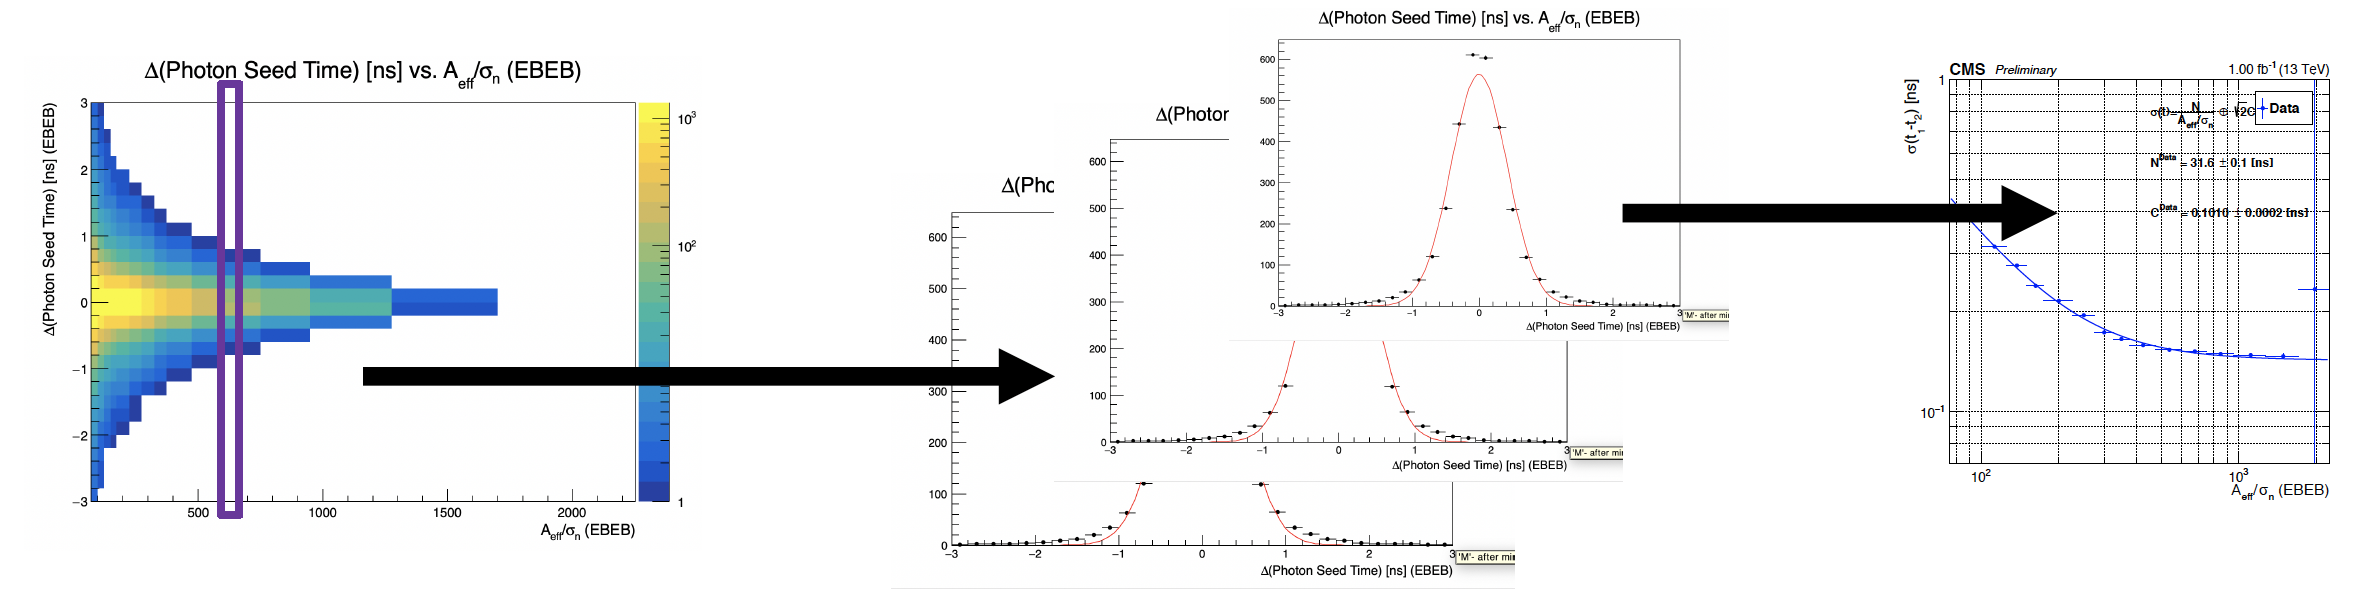
\includegraphics{fig/sec_method/timeres_process.png}}
\caption{To measure the time resolution the $\Delta(Seed Time)$ is plotted in bins of $A_{eff}/\sigma_{N}$.  The distribution of $\Delta(Seed Time)$ in each bin is plotted and fit to a Gaussian to extract the standard deviation, $\sigma(t_{1}-t_{2})$, of the distribution.  The $\sigma(t_{1}-t_{2})$ for the distribution in each bin is plotted in bins that are the same as the bin from which it was derived.  The resulting plot is fitted as a function of $A_{eff}/\sigma_{N}$ as shown in Equation 5.}
\label{trm_timeproccess}
\end{center}
\end{figure}

\begin{equation}
    \sigma^{2}_{i} = (\frac{N}{A_{eff}/\sigma_{N}})^{2} + 2C^{2}\\
    \label{eq_b}
\end{equation}

The dependence of $\sigma(t_{1}-t_{2})$ on $A_{eff}/\sigma_{N}$ characterizes the time resolution. This dependence is traditionally fitted with the resolution function in Equation \ref{eq_b} for $A_{eff}/\sigma_{N} > 75$. In this equation the noise term ( N ) is the coefficient for the uncertainty due to noise and the constant term ( C ) has several contributions including the variability of the point of shower initiation within the crystal, systematic effects such as those due to small differences in pulse shapes in different crystals, differences in processing delays due to different readout electronics, and pileup effects.  The constant term is the resolution of the time reconstruction for the particular case ( same read-out unit, different read-out unit, $Z\rightarrow e^{+}e^{-}$ ) considered. 

\begin{equation}
    \sigma^{2}_{i} = (\frac{N}{A_{eff}/\sigma_{N}})^{2} + \frac{S^{2}}{A_{eff}/\sigma_{N}} + 2C^{2}\\
    \label{eq_c}
\end{equation}

%The fits for these resolutions where preformed with the addition of a stochastic term as shown here :
As shown in Equation \ref{eq_c} the parameterization for the resolution can be extended with the inclusion of a stochastic term ( S ). While a stochastic term is not traditionally used, the inclusion of this term improved the fits when the limit $A_{eff}/\sigma_{N} $ is lowered to 10 to better characterize the shape of the low energy dependance. This approach in taken for the resolutions of the time reconstruction using the CC method.

\hfill
\begin{table}[h!]
\begin{center}
 \begin{tabular}{ |c| }
 \hline
 Resolution Selection Cuts \\
 \hline
 \hline
 Local Resolution\\
 \hline
  %isOOT false \\
  %At least one photon candidate \\
  Photon smin $>$ 0.3 \\
  Photon smaj $>$ 0.5 \\
  %choose a seed crystal and an adjacent crystal to the seed crystal\\ 
  Photon seed crystal has an adjacent crystal where : \\ 
  seed crystal energy $<$ 120\% adjacent crystal energy \\
  Qualifying seed crystal with largest energy \\
 \hline
 Global Resolution\\
 \hline
  Photon has PixSeed \\
  Photon gedID $<$ 3 \\
  %isOOT false \\
  Photon matches to an electron with dR $<$ 0.1  \\
  Matching electron has trackZ within 1.0 cm of primary vertex Z \\
  At least 2 qualifying photons \\
  Pair of photons with combined mass $<$ 150 GeV \& $>$ 60 GeV \\
  Qualifying pair of photons with combined mass closets to Z mass \\
\hline
\end{tabular}
\end{center}
\caption{Selection cuts for local and global resolutions.}
\label{res_params}
\end{table}


%\begin{figure}[htbp]
%\begin{center}
%\resizebox{0.41\textwidth}{!}{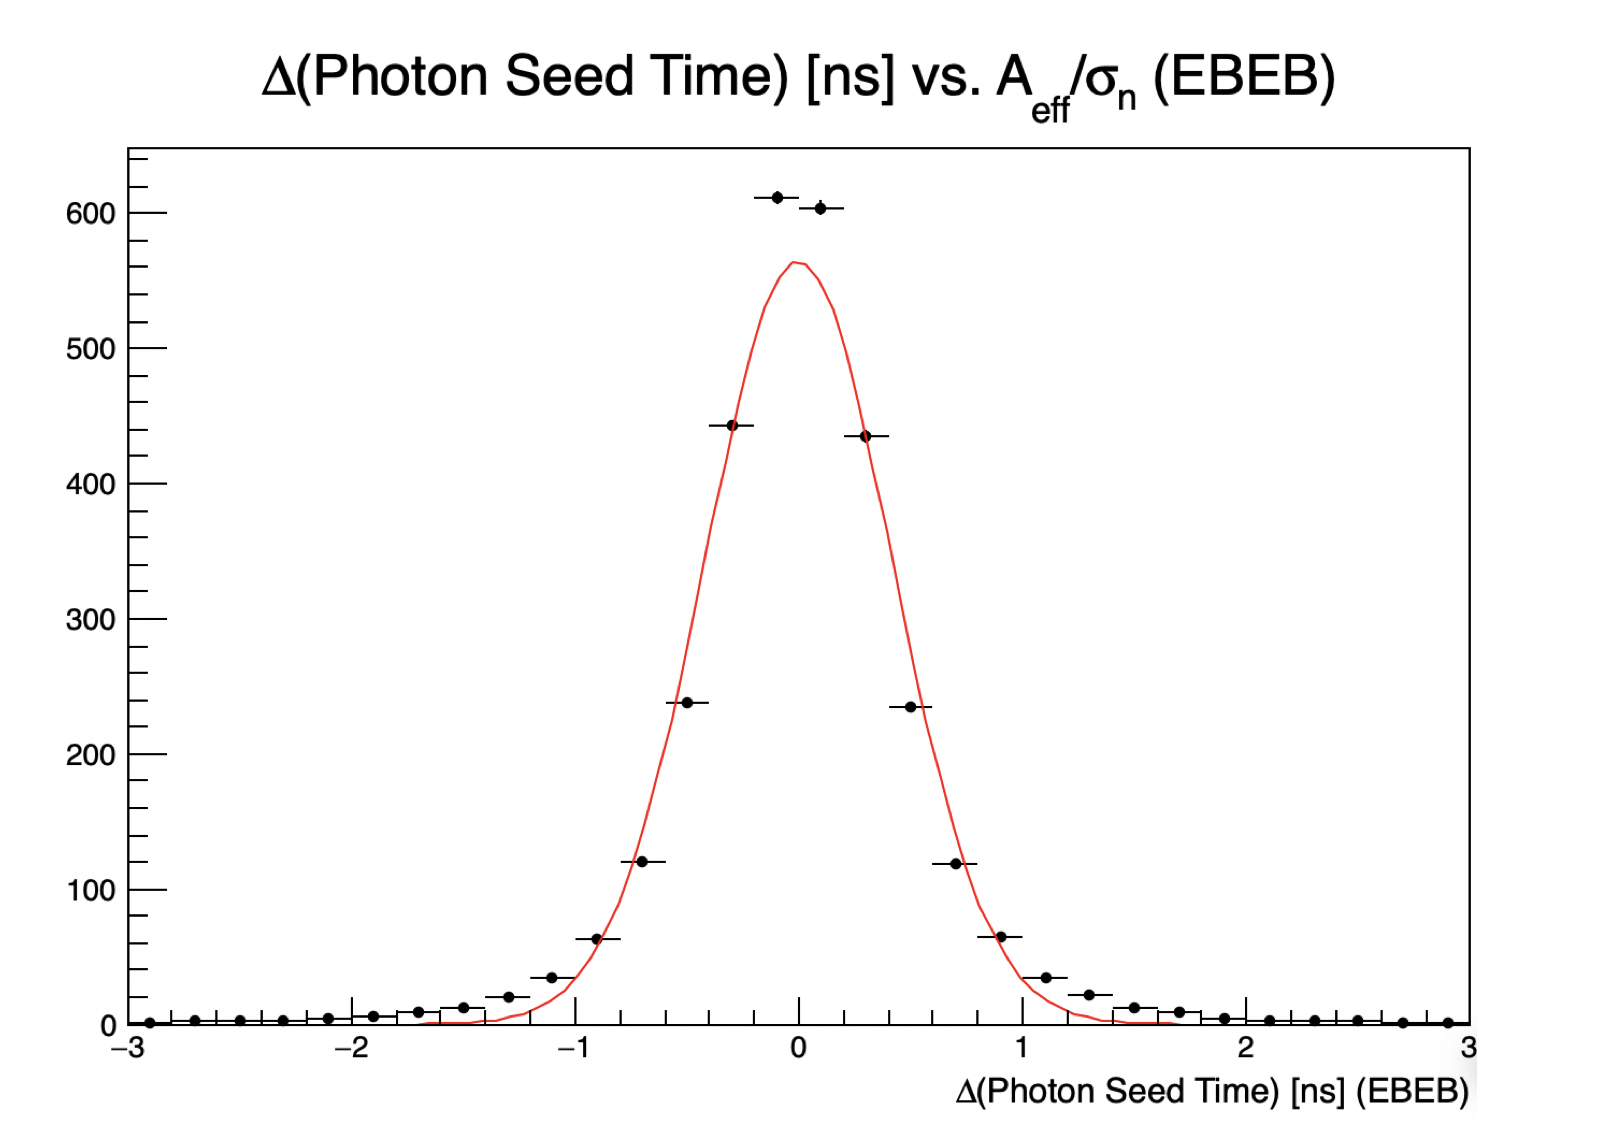
\includegraphics{fig/sec_method/timedis_fit.png}}
%\resizebox{0.33\textwidth}{!}{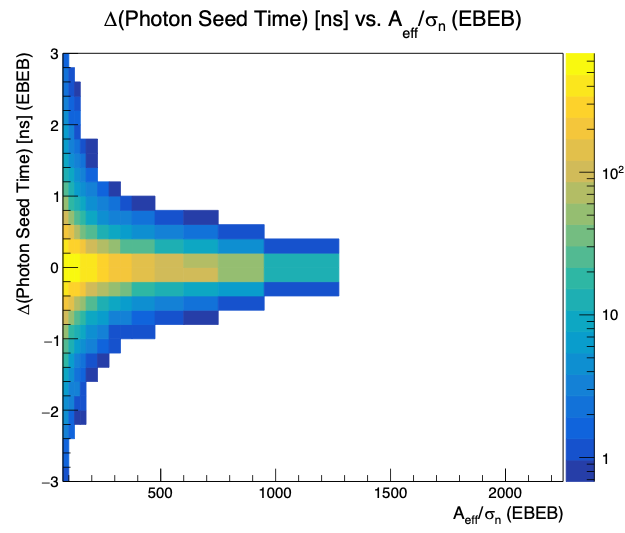
\includegraphics{fig/sec_method/deltime_v_effA.png}}
%\caption{The plot on the left shows the distribution of time differences for the crystal pairs, $\Delta(Photon Seed Time)$, plotted in bins of effective amplitude, $A_{eff}/\sigma_{N}$.  The plot on the right shows the Gaussian fit of a distribution of $\Delta(Photon Seed Time)$ in a single bin of $A_{eff}/\sigma_{N}$.} 
%\label{trm_dtplots}
%\end{center}
%\end{figure} 